\documentclass[a4paper, 12pt]{article}
\usepackage[utf8]{inputenc}
\usepackage{myshortcuts}
\usepackage{a4wide}
\usepackage{mhchem}
\usepackage{physics}
\usepackage{csquotes}
\usepackage{enumitem}
\usepackage{etoolbox}
\usepackage{multirow}
\usepackage[british]{babel}
\usepackage[labelfont=bf]{caption}
\usepackage[style=numeric,backend=biber]{biblatex}
\usepackage[separate-uncertainty=true, multi-part-units=single]{siunitx}

\allowdisplaybreaks

\sisetup{detect-all = true}

\DeclareSIUnit{\molar}{M}

% https://tex.stackexchange.com/questions/201425/command-to-italicize-text-with-slanted-numbers

\addbibresource{mysources.bib}

\title{
\textbf{Chemistry Internal Assessment}\\
\bigskip
What effect does varying the concentration have on the rate of decomposition of \ce{H2O2} in presence of \ce{Fe^3+} ions?
}
\author{}
\date{}

\begin{document}
\maketitle

\section*{Background Information}
$$\ce{2 H2O2(aq) ->[{cat.}] 2 H2O(l) + O2(g)}$$
...

\section*{Research Question}
...
\paragraph{Hypothesis} ...

\section*{Variables}
\paragraph{Independent variable:}
concentration of \ce{H2O2}

\paragraph{Dependent variable:}
initial rate of change in gas pressure

\paragraph{Controlled variables:}
\begin{itemize}
    \itemsep 0em
    \item volume of reaction mixture
    \item concentration of \ce{FeCl3} catalyst
    % TODO check if these should be included if to be talked in evaluation
    \item temperature of reaction mixture
    \item volume of test tube
\end{itemize}

\section*{Materials}
\subsection*{Apparatus}
\begin{itemize}
    \itemsep 0em
    \item \SI{1}{\L} beaker
    \item \SI{18x150}{\mm} glass test tubes
    \item one-hole rubber stopper
    \item tubing with two Luer-lock connectors
    \item LabQuest
    \item Vernier temperature probe (range: \num{-40} to \SI{135}{\celsius}; accuracy: \SI{+-0.2}{\celsius} \autocite{vernier_temperature})
    \item Vernier gas pressure sensor (range: \num{0} to \SI{210}{\kPa}; accuracy: \SI{+-4}{\kPa} \autocite{vernier_gas_pressure})
    \item three \SI{5.00}{\mL} graduated pipettes (precision: \SI{+-0.05}{\mL}) with bulbs
\end{itemize}

\subsection*{Chemicals}
\begin{itemize}
    \itemsep 0em
    \item \SI{80}{\mL} of \SI{3}{\percent}(w/w) \ce{H2O2}
    \item \SI{30}{\mL} of \SI{0.1}{\molar} \ce{FeCl3}
    \item \SI{80}{\mL} of distilled water
\end{itemize}
\paragraph{Safety} 
Although \SI{3}{\percent} \ce{H2O2} is classified as non-hazardous \autocite{safety_h2o2}, \SI{0.1}{\molar} \ce{FeCl3} is identified to be irritant and corrosive upon immediate skin or eye contact \autocite{safety_fecl3}. Goggles, gloves, and a lab coat must be worn.

\section*{Method}
\begin{enumerate}
    \itemsep 0em
    \item Set up a water bath with a \SI{1}{\L} beaker to immerse a test tube with room-temperature water --- see \cref{fig:setup} below.
    \item Connect the rubber stopper to a Vernier gas pressure sensor with a plastic tubing, and secure with one-half turn of the fittings.
    \item \label{item:trial-start} Using graduated pipettes, draw \SI{1.00}{\mL} of \SI{3}{\%} hydrogen peroxide and \SI{3.00}{\mL} of distilled water into the test tube.
    \item Record the temperature of the water using a temperature probe. Wait for 5 minutes until the solution in the test tube reaches the same temperature as the bath.
    \item Connect the gas pressure sensor and the temperature probe to a LabQuest. Set up the LabQuest to record 2 samples per second for 180 seconds.
    \item Using another graduated pipette, draw \SI{1.00}{\mL} of \SI{0.1}{\molar} iron(III) chloride solution. The concentration of the catalyst is then $[\ce{Fe^3+}] = \SI{1.0}{\molar} \times \frac{ \SI{1.00}{\mL} }{ \SI{5.00}{\mL} } = \SI{0.02}{\molar}$.
    \item Remove the rubber stopper. Quickly transfer the aqueous catalyst from the pipette to the test tube. Shake to mix the substances. Seal the test tube with the rubber stopper, and start recording data.
    \item \label{item:trial-end} Carefully remove the stopper to release the gas produced. Dispose of the solution in a labelled jar for metal waste, and rinse the test tube. Save the experimental data.
    \item \label{item:trials-end} Repeat steps \ref{item:trial-start} to \ref{item:trial-end} for at least another two trials.
    \item Repeat steps \ref{item:trial-start} to \ref{item:trials-end}, increasing the volume of hydrogen peroxide added in step \ref{item:trial-start} by \SI{0.50}{\mL} up to \SI{4.00}{\mL} and decreasing the volume of distilled water by \SI{0.50}{\ml}.
\end{enumerate}
\paragraph{Disposal} Excess \ce{H2O2} can go down the sink with water; leftover \ce{FeCl3} must be discarded in the metal waste jar. Unused \ce{H2O2} should be stored in a refrigerator.

\begin{figure}[H]
    \centering
    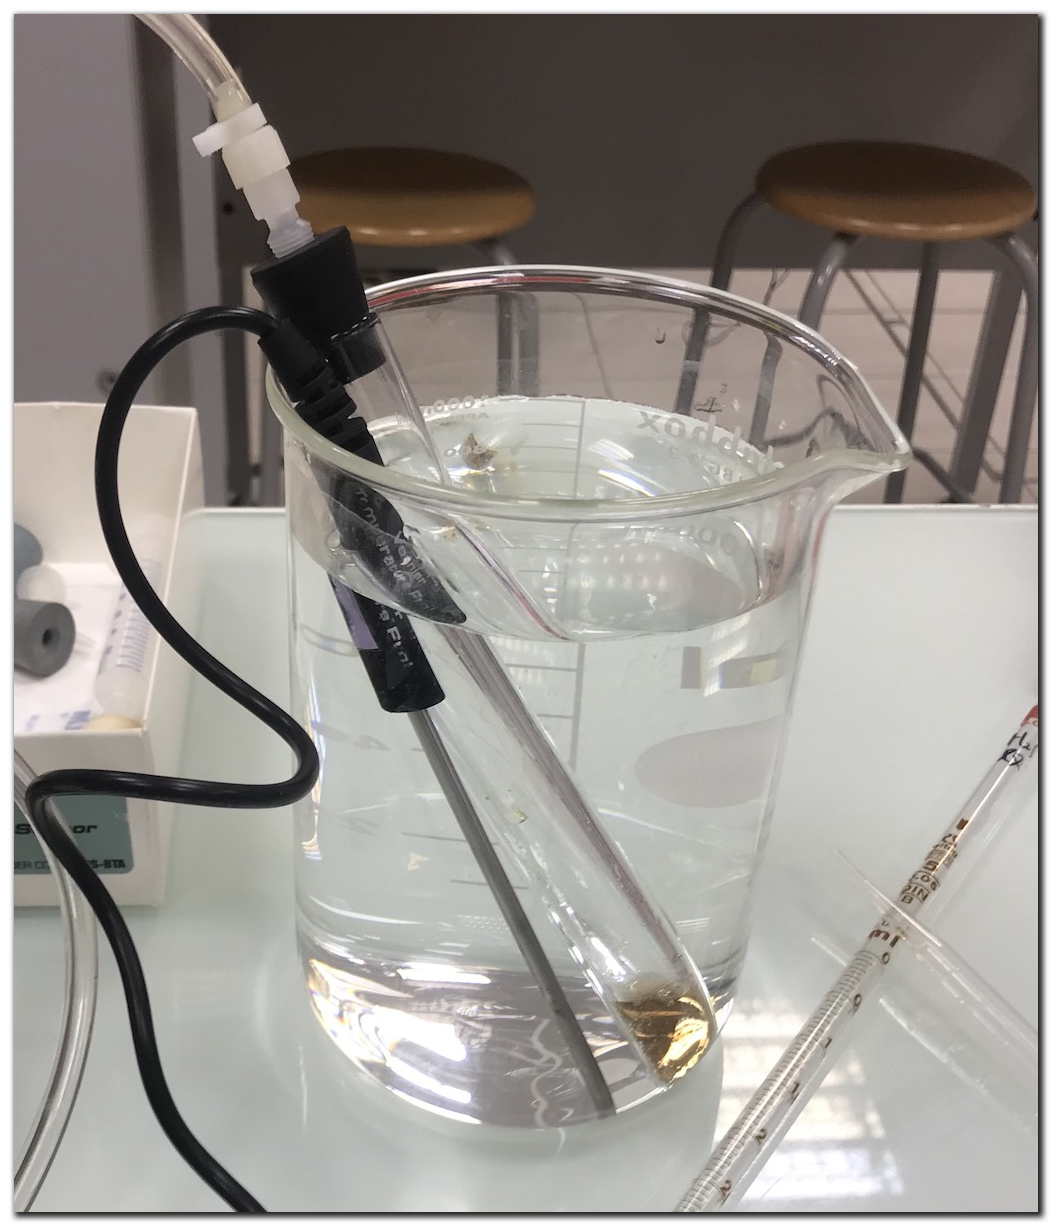
\includegraphics[width=0.36\textwidth]{imgs/setup}
    \caption{Setup of the experiment}
    \label{fig:setup}
\end{figure}


\section*{Raw Data}
\subsection*{Observations}
\begin{itemize}
    \itemsep 0em
    \item \SI{3}{\percent} \ce{H2O2} is a clear, colourless solution. Some fine bubbles can be seen.
    \item Upon the addition of \SI{0.1}{\molar} \ce{FeCl3}, the aqueous catalyst turns from pale yellow to brown, accompanied by a vigorous effervescence after shaking.
    \item 2 trials using \SI{4.00}{\mL} \ce{H2O2} were terminated prematurely, because the rubber stopper popped due to an excessive volume of gas formed.
    \item After about 10 minutes, with the formation of gas becoming less noticeable, the pale yellow colour of \ce{FeCl3} solution returns.
\end{itemize}

\begin{figure}[H]
    \centering
    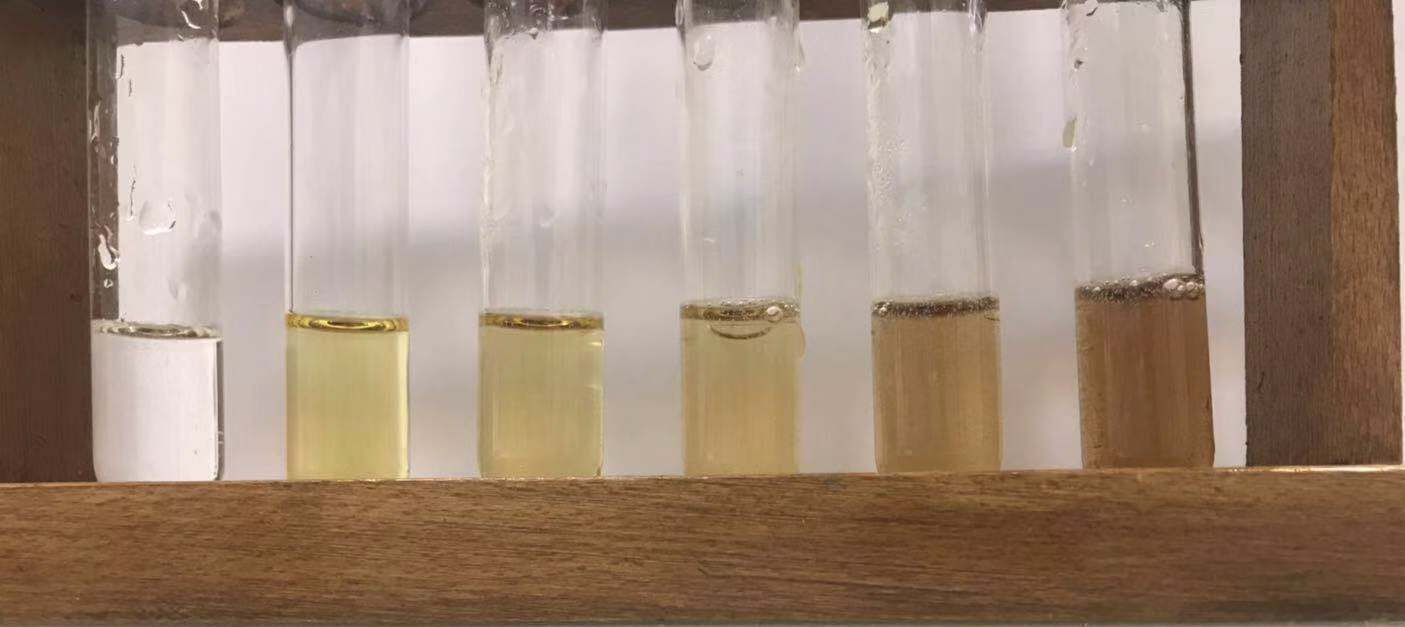
\includegraphics[width=0.8\textwidth]{imgs/colours}
    \caption{(From left to right) hydrogen peroxide, iron(III) chloride, reaction mixtures approximately 12 minutes, 9 minutes, 6 minutes, and 3 minutes after the start of reaction. }
    \label{fig:colours}
\end{figure}

\subsection*{Experimental data}
\begin{figure}[H]
    \centering
    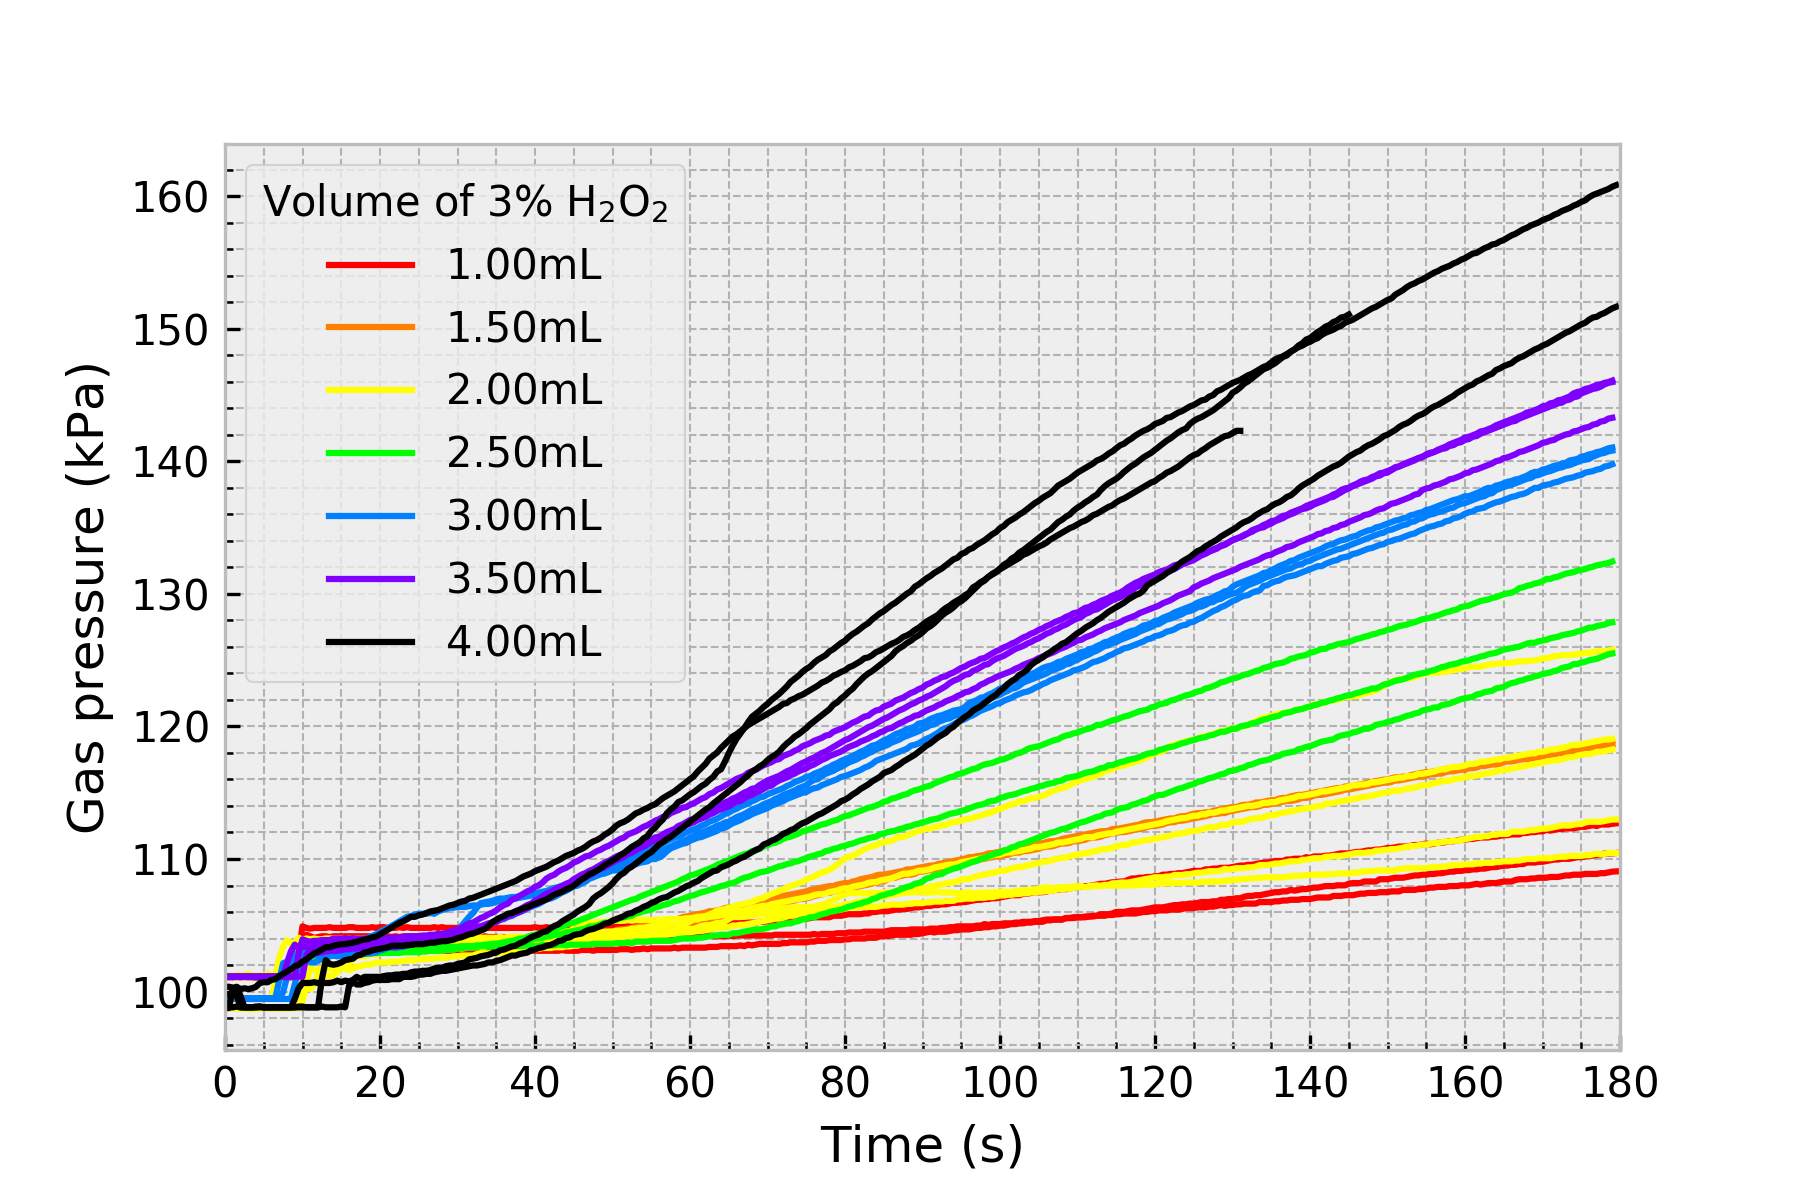
\includegraphics[width=\textwidth]{data/raw_data}
    \caption{Measured gas pressure over time for the decomposition of \ce{H2O2} by \ce{Fe(III)}. $[\ce{Fe^{3+}}] = \SI{0.02}{\molar}$; ambient temperature (\SI{23.3(10)}{\celsius}). }
    \label{fig:raw-data}
\end{figure}

The gas pressure curve generally consists of 3 parts: an initial plateau before sealing the test tube, a slowly increasing curve after inserting the rubber stopper which can be attributed to the dissolution of the oxygen produced, and a linear part where the aqueous oxygen reaches saturation and gaseous oxygen continues to be produced at a mostly consistent rate. Overall, the larger the volume and as such the higher concentration of the \ce{H2O2} is reacted, the larger the volume of oxygen gas is formed as measured by the gas pressure at each instant. A deviation from this trend occurs for \SI{2.00}{\mL} of \ce{H2O2}, which may be attributed to the fact that, unlike the other trials, those 4 were all carried out next to the window on a cold winter day.

\section*{Processed Data}
Below is a sample calculation for the trials with \SI{3.00}{\mL} of \ce{H2O2} shown by the blue curves in \cref{fig:raw-data}. The initial rate is derived from the first \SI{15}{\s}-long segment of the linear part --- determined by the R$^2$ value of the line of best fit --- using the differential formula \autocite{numerical_method}:
\[ 
    \dv{P}{t} 
    = \dfrac{ P_{ \text{end} } - P_{ \text{start} } }{ t_{ \text{end} } - t_{ \text{start} } }
    \text{ where } t_{ \text{end} } - t_{ \text{start} } = \SI{15.00}{\s}. 
\]

\begin{table}[H]
    \centering
    \caption{Initial rates for reactions with \SI{3.00}{\mL} of \SI{3}{\%} \ce{H2O2}}
    \label{table:calc}
    \begin{tabular}{ | c | c | c | c | }
        \hline
        \multirow{2}{*}{\textbf{Trials}} &
        \multicolumn{2}{ c| }{\textbf{Gas pressure (\si{\kPa})}}& 
        \multirow{2}{*}{\textbf{Initial rate (\si{\kPa\per\second})}}
        \\ \cline{2-3}
        &
        $t = \SI{91.5}{\second}$ &
        $t = \SI{121.5}{\second}$ &
        \\ \hline
        0 &
        113.96 &
        117.80 &
        0.256
        \\ \hline
        1 &
        119.06 &
        123.19 &
        0.275
        \\ \hline
        2 &
        120.38 &
        124.40 &
        0.268
        \\ \hline
        3 &
        119.92 &
        123.88 &
        0.264
        \\ \hline
        \multicolumn{3}{ | c | }{\textbf{Average}} &
        0.269
        \\ \hline
        \multicolumn{3}{ | c | }{\textbf{Standard deviation}} &
        0.003
        \\ \hline
    \end{tabular}
\end{table}

Note that the accuracy of \SI{\pm 4}{\kPa} of the gas pressure sensor is considered to affect the readings consistently, and as such is a systematic error that does not contribute to the uncertainty in the initial rate. Furthermore, the uncertainties arising from the precision of the readings evaluates to 
\begin{align*}
    \Delta \left(\dv{P}{t}\right) 
    &=  \dv{P}{t} 
        \times \left(
            \frac{ 2 \times \SI{0.01}{\kPa} }{P_{ \text{end} } - P_{ \text{start} }}
            + \frac{ 2 \times \SI{0.01}{\s} }{t_{ \text{end} } - t_{ \text{start} }}
        \right)\\
    &= \SI{0.269}{\kPa\per\s} \times \left( \frac{\SI{0.02}{\kPa}}{\SI{0.269}{\kPa\per\s} \times \SI{15.00}{\s}} + \frac{\SI{0.02}{\s}}{\SI{15.00}{\s}} \right)\\
    &= \SI{+-0.002}{\kPa\per\s}
\end{align*}
which is smaller than --- or even negligible for some other trials --- the standard deviation. Therefore, the uncertainty in the initial rate is determined by the standard deviation.

The \SI{3}{\%}(w/w) concentration of \ce{H2O2} means that, proportionally, there is \SI{3}{\g} of \ce{H2O2} per \SI{100}{\g} of solution. In addition, it is indicated on the data sheet \autocite{safety_h2o2} that the density of the solution is \SI{1.01}{\g\per\cm^3}. The molar concentration of the \SI{3}{\%}(w/w) \ce{H2O2} solution is then
\begin{align*}
    % Initial concentration
    [\ce{H2O2}]_{\SI{3}{\%}}
    &= \dfrac{ n(\ce{H2O2}) }{ V(\text{solution}) }\\
    &= \dfrac{ m(\ce{H2O2}) / RFM(\ce{H2O2}) }{ m(\text{solution}) / \rho(\text{solution})}\\
    &= \dfrac{ \SI{3}{\g} / \SI{34.02}{\g\per\mol} } { \SI{100}{\g} / \SI{1.01}{\g\per\cm\cubed} }\\
    &= \SI{8.91E-4}{\mol\per\cm\cubed}\\
    &= \SI{0.891}{\molar}.\\
    % Diluted concentration
    [\ce{H2O2}]
    &= [\ce{H2O2}]_{\SI{3}{\%}} \times \dfrac{ V(\ce{H2O2}) }{ V(\ce{H2O2}) + V(\ce{H2O}) + V(\ce{FeCl3}) }\\
    &= \SI{0.891}{\molar} \times \dfrac{ \SI{3.00}{\mL} }{ \SI{3.00}{\mL} + \SI{1.00}{\mL} + \SI{1.00}{\mL} }\\
    &= \SI{0.534}{\molar}\\
    % Uncertainty in diluted concentration
    \Delta([\ce{H2O2}])
    &= [\ce{H2O2}] \times \fracDeltaP{\ce{H2O2}}\\
    &= [\ce{H2O2}] \times \left(\fracDelta{V(\ce{H2O2})} + \frac{ \Delta V(\ce{H2O2}) + \Delta V(\ce{H2O}) + \Delta V(\ce{FeCl3}) }{ V(\ce{H2O2}) + V(\ce{H2O}) + V(\ce{FeCl3}) }\right)\\
    &= \SI{0.534}{\molar} \times \left(\frac{ 2 \times \SI{0.05}{\mL} }{ \SI{3.00}{\mL} } + \frac{ 2 \times \SI{0.05}{\mL} + \SI{0.05}{\mL} + \SI{0.05}{\mL} }{ \SI{3.00}{\mL} + \SI{1.00}{\mL} + \SI{1.00}{\mL} }\right)\\
    &= \SI{+-0.039}{\molar}
\end{align*}

The figures are calculated in the same figure for the other trials, yielding:

\begin{table}[H]
    \centering
    \caption{Initial rate versus [\ce{H2O2}]. The sample calculation is highlighted in italics. }
    \label{table:data}
    \begin{tabular}{ | c | c | }
        \hline
        \textbf{[\ce{H2O2}]} (\si{\molar}) &
        \textbf{Average initial rate} (\si{\kPa\per\second})
        \\ \hline
        \num{0.178(24)} & \num{0.063(12)}
        \\ \hline
        \num{0.267(28)} & \num{0.106(1)}
        \\ \hline
        \num{0.356(32)} & \num{0.101(49)}
        \\ \hline
        \num{0.445(35)} & \num{0.193(12)}
        \\ \hline
        \textit{\num{0.534(39)}} & \textit{\num{0.269(3)}}
        \\ \hline
        \num{0.623(42)} & \num{0.291(6)}
        \\ \hline
        \num{0.713(46)} & \num{0.366(35)}
        \\ \hline
    \end{tabular}
\end{table}

\section*{Results}
Two kinetic models are proposed for explaining the experimental data: the rate equation given by a power law, and the Michaelis-Menten equation.

\paragraph{Rate equation}
This approach assumes that, like for many reactions, the rate equation of the reaction $\ce{ 2 H2O2(aq) ->[Fe^3+] 2 H2O(l) + O2(g) }$ is given by the power law
\[ \text{rate} = \dv{[\ce{O2(g)}]}{t} = k [\ce{H2O2}]^a [\ce{Fe^3+}]^b. \]
Since [\ce{Fe^3+}] is held constant at \SI{0.02}{\molar}, the above rate equation can be expressed as 
\[ \dv{[\ce{O2(g)}]}{t} = k_{\text{obs}} [\ce{H2O2}]^a \]
where $k_{\text{obs}} = k \times [\ce{Fe^3+}]^b$. Additionally, supposing that the \ce{O2(g)} produced obeys the ideal gas law $P V = n R T$, it can be deduced that $P = \frac{n}{V} \times R T = [\ce{O2(g)}] \times R T$, with $V$ the volume of the test tube being constant. Thus, treating $T$ as a constant,
\begin{align}
    &\dv{P}{t} = \dv{[\ce{O2(g)}]}{t} \times R T \nonumber\\
    \iff &\dv{P}{t} = k_\text{obs} [\ce{H2O2}]^a \times R T \nonumber\\
    \iff &\dv{P}{t} = k_\text{obs}' [\ce{H2O2}]^a \text{ where } k_\text{obs}' = k_\text{obs} \times R T.\label{eq:rateEq}
\end{align}
The parameters $a$ and $k_{\text{obs}}'$ can then be determined using MATLAB's curve fitting toolbox.

\paragraph{Michaelis-Menten equation}
This approach is typically applied to model single-substrate enzyme-catalysed reactions, namely, the sequence of elementary reactions
\[
\ce{E + S <=>[ k_f ][ k_r ] ES ->[ k_{\text{cat}} ] E + P}
\]
where \ce{E}, \ce{S}, and \ce{P} are respectively the enzyme, the substrate, and the product. In this study, it is hypothesised that \ce{Fe^3+}, \ce{H2O2}, and \ce{O2} respectively play these roles.

Since the enzyme acts as a catalyst and is not consumed during the course of the reaction, it is admitted that $\ce{[E]_0} = \ce{[E] + [ES]}$ where $\ce{[E]_0}$ is the initial enzyme concentration, or equivalently, 
\[
\ce{[E]} = \ce{[E]_0 - [ES]}.
\]

A quasi-steady-state is assumed; i.e., 
\begin{align*}
    &\ce{k_f [E][S] - k_r [ES] - k_{\text{cat}} [ES] = 0}\\
    \iff &\ce{k_f ([E]_0 - [ES]) [S] - (k_r + k_{\text{cat}}) [ES] = 0}\\
    \iff &\ce{k_f [E]_0 [S] = (k_f [S] + k_r + k_{\text{cat}})[ES]}\\
    \iff &\ce{[ES] = \frac{k_f [E]_0 [S]}{k_f [S] + (k_r + k_{\text{cat}})}}
    = \ce{\frac{[E]_0 [S]}{[S] + K_m}}
\end{align*}
where $K_m = \dfrac{k_r + k_\text{cat}}{k_f}$ is known as the Michaelis constant. Finally, from $\ce{ES ->[k_{\text{cat}}] E + P}$, the rate of product of product formation is given by
\begin{align}
    \dv{\ce{[P]}}{t} &= k_{\text{cat}} \times \ce{[ES]} = k_{\text{cat}} \times \frac{\ce{[E]_0[S]}}{\ce{[S]} + K_m}
\nonumber\\
    \dv{P}{t} &= k_{\text{obs}} \times \frac{\ce{[S]}}{\ce{[S]} + K_m}\label{eq:mm}
\end{align}
where $k_{\text{obs}} = k_\text{cat} \ce{[E]_0} \times R T$. The parameters $k_{\text{obs}}, K_m$ along with an y-intercept to account for systematic errors are then determined using MATLAB's curve fitting toolbox.

\begin{figure}[H]
    \centering
    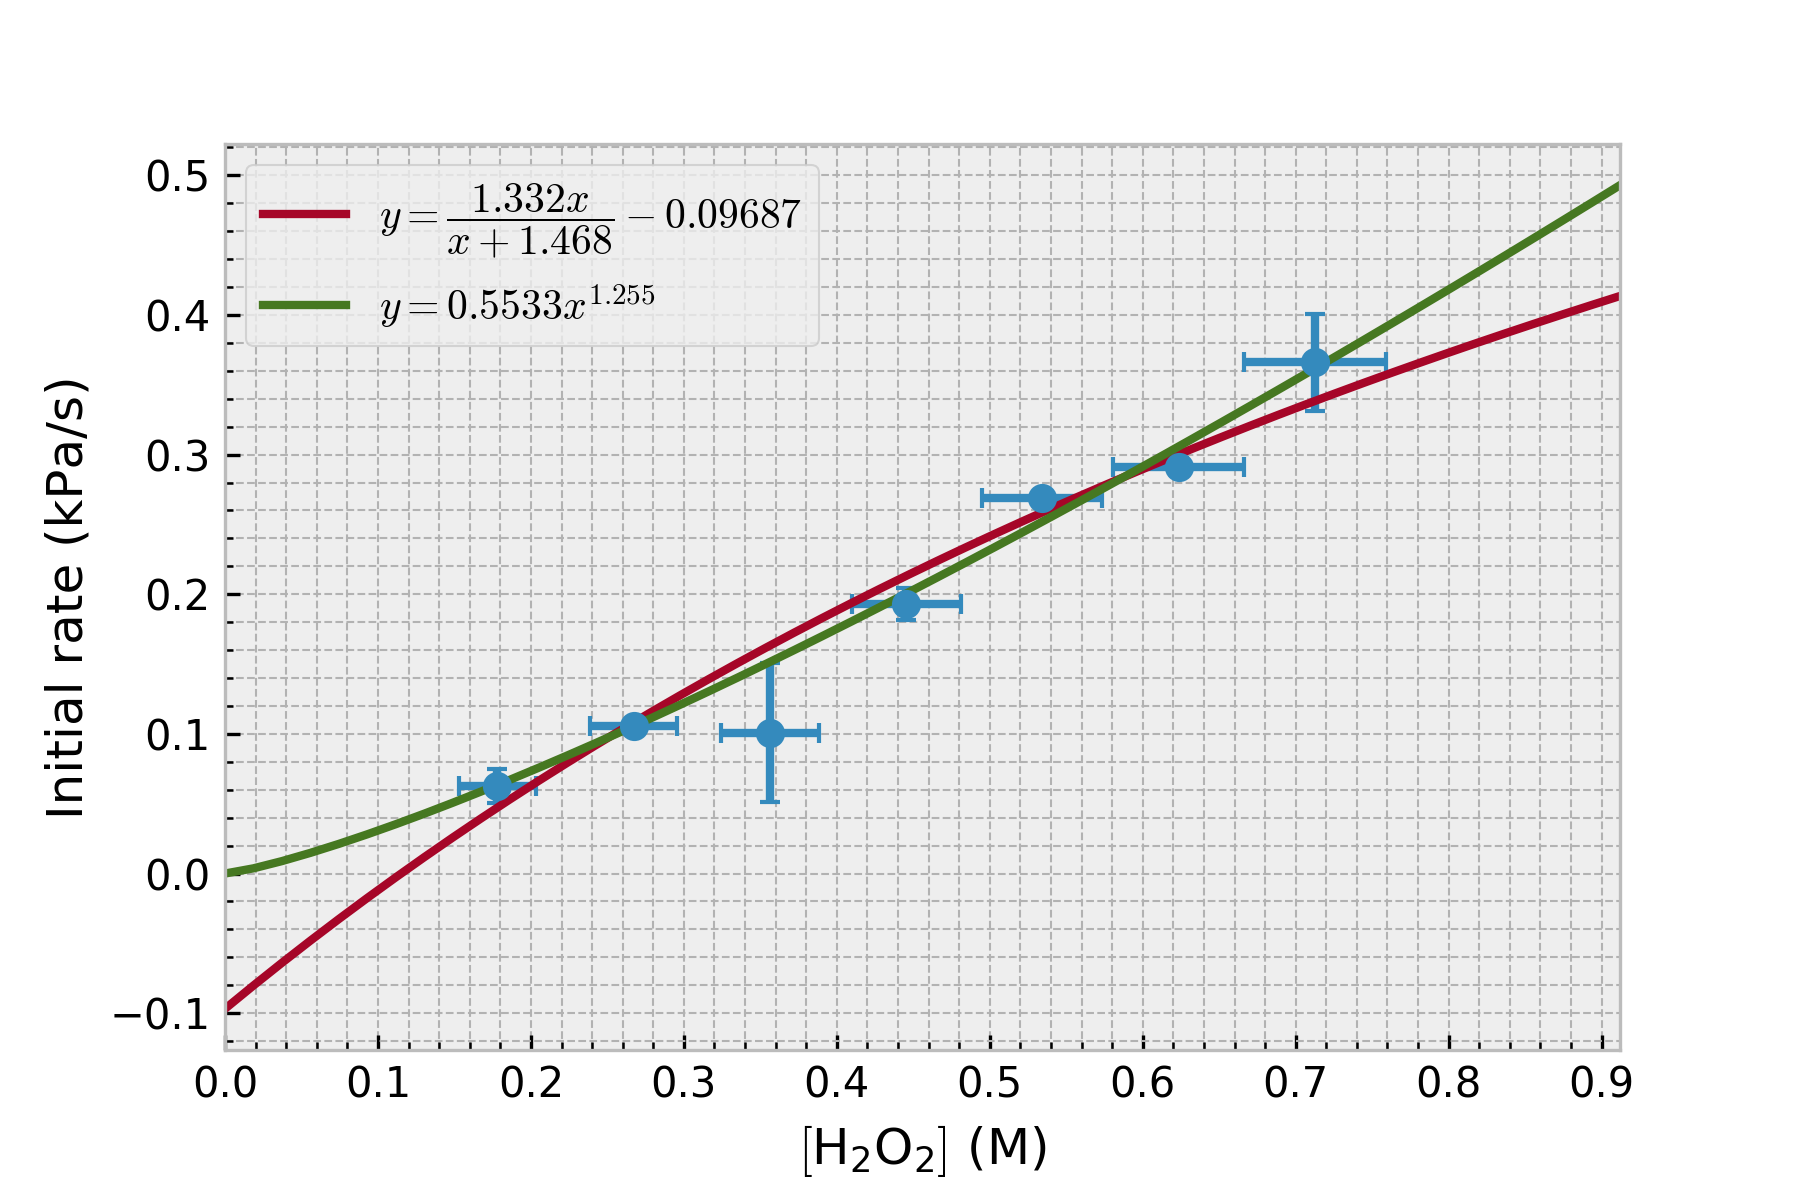
\includegraphics[width=\textwidth]{data/processed_data}
    \caption{Initial rate versus [\ce{H2O2}]. [\ce{Fe^3+}] = \SI{0.02}{\molar}; ambient temperature (\SI{23.3(10)}{\celsius}). \Cref{eq:rateEq}, the rate equation is shown in green; \cref{eq:mm}, the Michaelis-Menten equation, is shown in red. }
    \label{fig:processed-data}
\end{figure}



\section*{Evaluation}

\section*{Conclusion}

\section*{Extension}

\printbibliography

\end{document}
